%%%%%%%%%%%%%%%%%%%%%%%%%%%%%%%%%%%%%%%%%%%%%%%%%%%%%%%%%%%%%%%
%
% Welcome to Overleaf --- just edit your LaTeX on the left,
% and we'll compile it for you on the right. If you open the
% 'Share' menu, you can invite other users to edit at the same
% time. See www.overleaf.com/learn for more info. Enjoy!
%
%%%%%%%%%%%%%%%%%%%%%%%%%%%%%%%%%%%%%%%%%%%%%%%%%%%%%%%%%%%%%%%
\documentclass[unicode,11pt]{beamer}
\usepackage[whole,autotilde]{bxcjkjatype}
\usetheme{Madrid}
\definecolor{links}{HTML}{2A1B81}
\hypersetup{colorlinks,linkcolor=,urlcolor=links}

\title{システム情報工学特論}
\subtitle{コードで学ぶAWS入門 - 第一回}
\author{真野智之 (Tomoyuki Mano)}
\institute[OIST]{Okinawa Institute of Science and Technology}
\date{2021/06/23 @東大工学部}

\begin{document}

\frame{\titlepage}

\begin{frame}{自己紹介}
真野智之 (Tomoyuki Mano)
\begin{itemize}
    \item 東京大学情報理工学系研究科システム情報学専攻博士課程修了 (2021年)
    \item 現職: 日本学術振興会特別研究員(PD),沖縄科学技術大学院大学フェロー
    \item 大学院時の研究: マウスの脳の三次元画像解析,クラウドを使ったデータベース構築
    \item 現在の研究: 頭足類(タコ・イカ) の脳の研究: 擬態(camouflage) を生み出す脳の神経回路を生成モデルの視点で解析したい
    (
    \href{https://twitter.com/CephWarden/status/1142083856893263872}{1},
    \href{https://twitter.com/CephWarden/status/1384644335069667334}{2},
    \href{https://twitter.com/CephWarden/status/1232307456346181632}{3}
    )
    \item 講義に関する質問などは次の連絡先まで. tomoyukimano@gmail.com
\end{itemize}
\end{frame}

\begin{frame}{成績評価}
\begin{itemize}
    \item 成績は期末レポート (課題内容は後日発表) で評価します
\end{itemize}
\end{frame}

\begin{frame}{講義について (1)}
\begin{itemize}
    \item 講義資料は
    \url{https://tomomano.github.io/learn-aws-by-coding/}\\
    にあります.
    \item ハンズオンで使用するソースコードは \url{https://github.com/tomomano/learn-aws-by-coding}\\
    にあります
    \item 課題やいくつかの補助スライドは
    \url{https://github.com/tomomano/intro-aws-2021}\\
    にあります
\end{itemize}
\end{frame}

\begin{frame}{講義について (2)}
\begin{itemize}
    \item 講義の中盤 (50分前後) で一度休憩をとります.
    この際に質問などにも答えます.
    \item 講義に関する質問は Zoom のチャットに飛ばして下さい.
    できるだけすぐにその場で回答します.
    \item 講義の内容は
    \url{https://tomomano.github.io/learn-aws-by-coding/}\\
    に従って行います.
    講義ではコードのデモなど行いますが,基本的に伝える情報は資料と同じです.
    余裕のある人は各自のペースでどんどん先に進んでしまって構いません.
    \item ハンズオンのプログラムでバグなど発見した場合は
    \href{https://github.com/tomomano/learn-aws-by-coding/issues}{GitHub の Issues}
    まで報告してもらえると助かります (残念ながら成績には関係ありません).
\end{itemize}

\end{frame}

\begin{frame}{講義の予定}
    \begin{itemize}
        \item 第一回 (6/23): イントロダクション (1章-3章),AWS Educate のアカウント準備
        \item 第二回 (6/30): クラウドを使った深層学習入門 part 1(4章-6章)
        \item 第三回 (7/7): クラウドを使った深層学習入門 part 2 (7章-9章)
        \item 第四回 (7/14): サーバーレス入門 (10章-13章)
    \end{itemize}
\end{frame}

\begin{frame}
\frametitle{AWS Educate のアカウントの用意 (1)}

\begin{itemize}
    \item 講義では実際に AWS のクラウドにアプリケーションを展開します.
    それには AWS Educate により提供されている学習用アカウントを使用します.
    本講義は AWS Educate プログラムに参加しているので,各アカウントには50ドル分のクーポン(利用枠)がついています.
    \item {\color{red} 期末レポート課題は各自の AWS Educate アカウントを使って実施してもらいます.
    期末時までに半分(25ドル)以上のクーポンを残しておいてください.
    もし足りなくなった場合はおかわり可能ですが,手続きが必要です.}
    \item まだ AWS Educate の招待が来ていない人は,今すぐ gcc のメールアドレスを連絡してください.
    \item この講義の前に AWS Educate に登録しているメールアドレスは拒否されるようです.
    その場合は代替のメールアドレス (gcc 以外も可) を連絡してください.
\end{itemize}

次からのスライドで示す手順でアカウントを取得します.

\end{frame}

\begin{frame}
\frametitle{AWS Educate のアカウントの用意 (2)}
\begin{itemize}
    \item アカウントの招待が gcc のメールアドレスに送られてきます.
    件名は "Your AWS Educate Application",差出人は "support@awseducate.com" のはずです.
    \item 招待のリンクに従ってアカウントを作ります.
    アカウントの承認に少し待たされます.
    \item アカウントが発行されたら, AWS Educate にログインしてください.
\end{itemize}

\begin{figure}
    \centering
    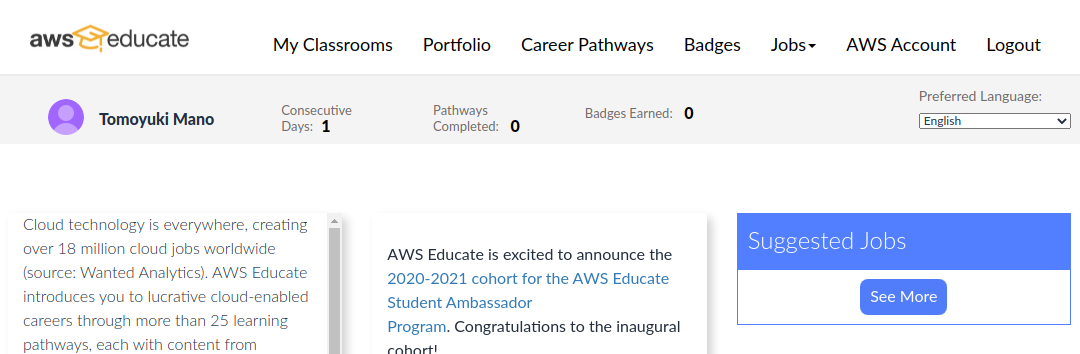
\includegraphics[width=0.5\textwidth]{imgs/aws_educate_screenshot1.png}
    \caption{AWS Educate ログイン画面}
\end{figure}

\end{frame}

\begin{frame}
\frametitle{AWS Educate のアカウントの用意 (3)}

\begin{itemize}
    \item AWS Educate のログイン画面のトップメニューバーから \emph{AWS Account} を開きます
    \item \emph{Create Starter Account} をクリックします
    \item 少し待つと Starter Account が作成されます
\end{itemize}

\begin{figure}
    \centering
    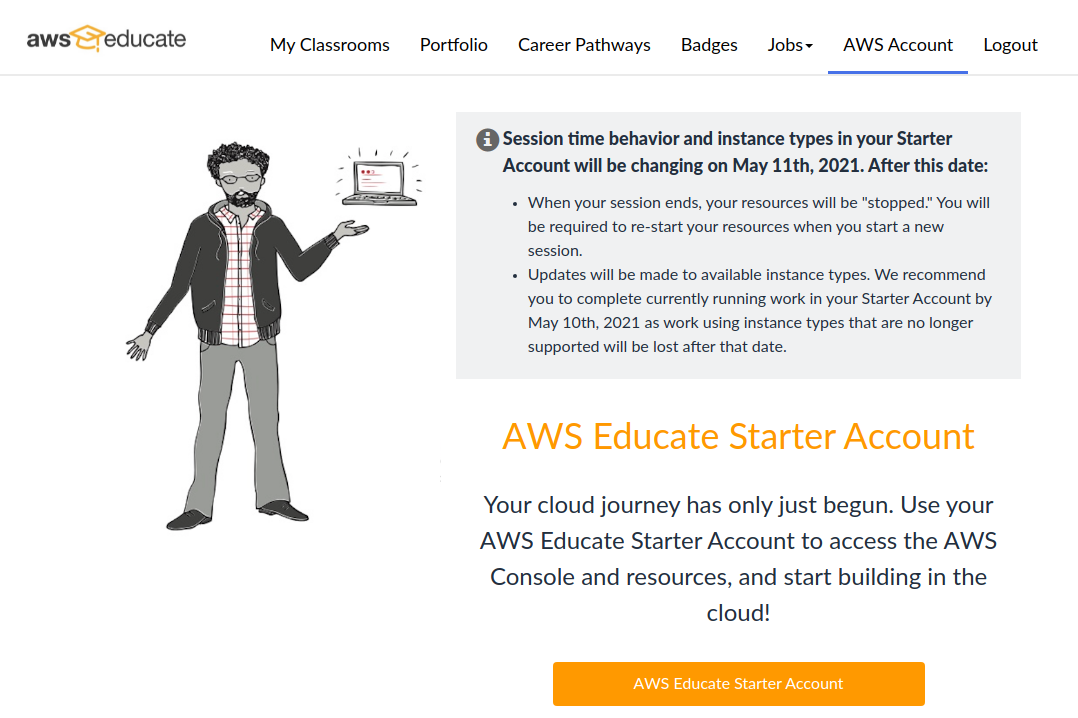
\includegraphics[width=0.5\textwidth]{imgs/aws_educate_screenshot2.png}
    \caption{AWS Educate Starter Account の作成}
\end{figure}

\end{frame}

\begin{frame}
\frametitle{AWS Educate のアカウントの用意 (4)}

\begin{itemize}
    \item \emph{AWS AWS Educate Starter Account} と書いてあるオレンジ色のボタンをクリックします
    \item vocareum (Starter account を提供しているサードパーティ会社) のサイトに飛び,利用規約が表示されます.
    熟読の上, \emph{I Agree} を押します.
    \item vocareum のコンソール画面が開きます.
\end{itemize}

\begin{figure}
    \centering
    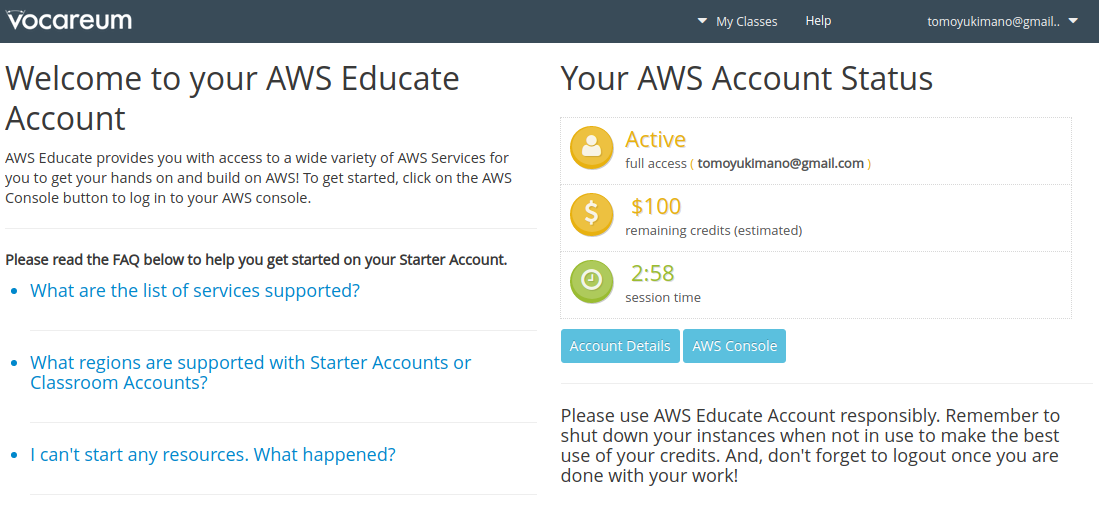
\includegraphics[width=0.5\textwidth]{imgs/vocareum_screenshot.png}
    \caption{vocareum のコンソール画面}
\end{figure}

\end{frame}

\begin{frame}
\frametitle{AWS Educate のアカウントの用意 (5)}

\begin{itemize}
    \item vocareum のコンソール画面から \emph{AWS Console} と書かれたボタンを押します.
    \item AWS コンソールが開きます
    \item このようにして得られた AWS アカウントを使って講義のハンズオンを実施してください.
\end{itemize}

\begin{figure}
    \centering
    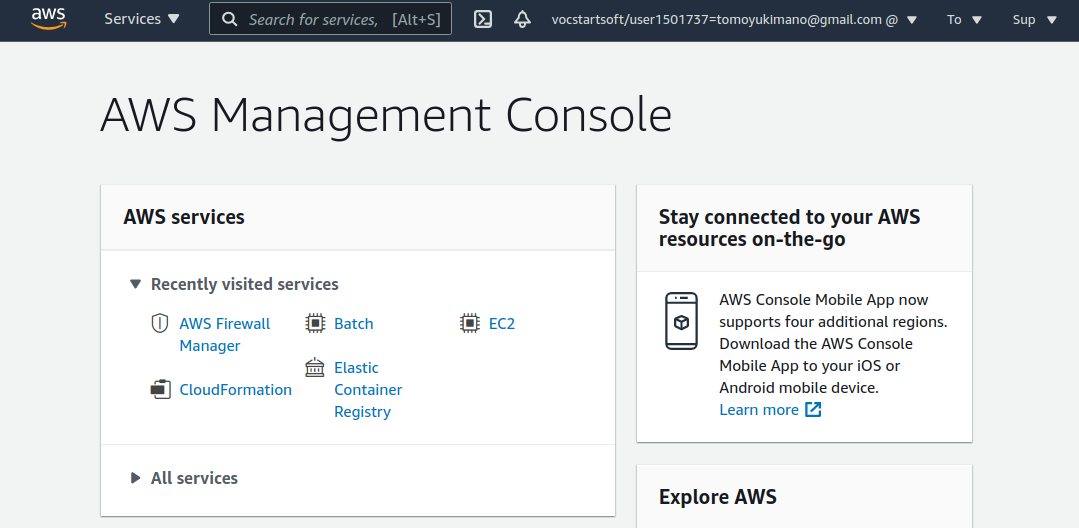
\includegraphics[width=0.5\textwidth]{imgs/aws_console_screenshot.png}
    \caption{AWS コンソール画面}
\end{figure}

\end{frame}

\begin{frame}{AWS Educate のシークレットキーの設定 (1)}

ここまでで AWS Educate Starter Account の取得が完了しました.

次にシークレットキーと呼ばれるものの設定を行います.
シークレットキーは, AWS CLI/CDK を使って AWS の API を操作する際の認証情報を担います.

Starter Account で作られたアカウントはシークレットキーの設定方法が一般アカウントと若干異なります.

次からのスライドで示す手順でシークレットキーを設定します.

\href{https://tomomano.github.io/learn-aws-by-coding/}{講義資料 (15章 Appendix)} にも同様の説明が記載されています.
    
\end{frame}

\begin{frame}{AWS Educate のシークレットキーの設定 (2)}

\begin{itemize}
    \item AWS Educate のコンソール画面から, vocareum のコンソールに移動します
    \item \emph{Account Details} をクリックし,続いて \emph{AWS CLI: Show} をクリックします
    \item \emph{aws\_access\_key\_id}, \emph{aws\_secret\_access\_key}, \emph{aws\_session\_token} が表示されます.ここで表示された内容を \emph{~\textasciitilde/.aws/credentials} にコピーします
\end{itemize}

\begin{figure}
    \centering
    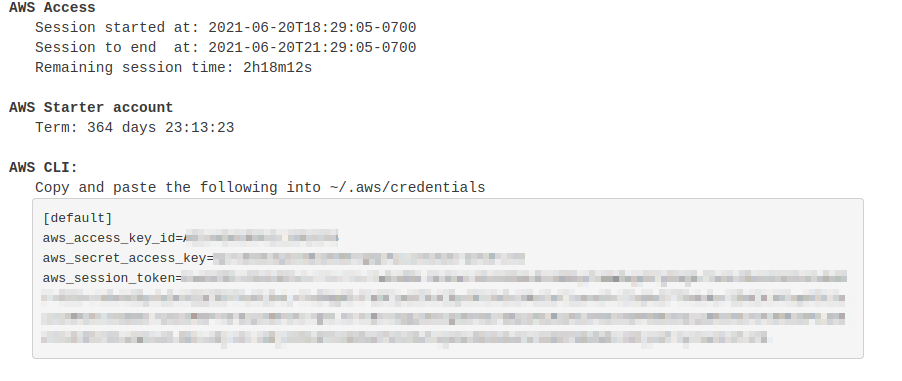
\includegraphics[width=0.5\textwidth]{imgs/vocareum_secret.png}
    \caption{vocareum から AWS シークレットキーの発行}
\end{figure}

\end{frame}

\begin{frame}[fragile]
\frametitle{AWS Educate のシークレットキーの設定 (3)}

\begin{itemize}
    \item 続いて, \emph{\textasciitilde/.aws/config} というファイルを用意し,次の内容を書き込みます.
    現時点では AWS Starter Account は \emph{us-east-1} リージョンでしか利用できないためです.
    
    \begin{semiverbatim}
    [profile default]
    region = us-east-1
    output = json
    \end{semiverbatim}
\end{itemize}

\end{frame}

\begin{frame}{AWS Educate のシークレットキーの設定 (4)}

\begin{itemize}
    \item ここまでの設定が正しくできているか以下の手順で確認します
    \item まずは AWS CLI をインストールします.
    \href{https://tomomano.github.io/learn-aws-by-coding/}{講義資料のAppendix}
    を参照
    \item コマンドラインから次のコマンドを実行します
    \begin{semiverbatim}
    aws ec2 describe-instances
    \end{semiverbatim}
    コマンドがエラーなく実行出来たら設定が正しく行われています
    \item \emph{An error occurred (ExpiredToken) when calling the ListBuckets operation: The provided token has expired.} というエラーが出た場合は?\\
    トークンの有効期限が切れています.
    もう一度 vocareum にログインしてシークレットキーを再発行してください.
    一般アカウントと違い, vocareum による Starter account は三時間ごとにキーが失効してしまいます.
\end{itemize}

\end{frame}

\end{document}

